\documentclass[10pt,a4paper]{article}
\usepackage[utf8]{inputenc}
\usepackage[italian]{babel}
\usepackage{amsmath}
\usepackage{amsfonts}
\usepackage{amssymb}
\usepackage{graphicx}
\usepackage{siunitx}
\usepackage{textcomp}
\usepackage[left=2cm,right=2cm,top=2cm,bottom=2cm]{geometry}
\newcommand{\rem}[1]{[\emph{#1}]}
\newcommand{\exn}{\phantom{xxx}}
\renewcommand{\thesubsection}{\thesection.\alph{subsection}}  %% use 1.a numbering

\author{Gruppo 1M.BB \\Simone Antognetti, Lorenzo Cavuoti, Fabrizio Chicconi}
\title{Ottica 1 - Misure con Spettroscopi}
\begin{document}
\date{17 Marzo 2019}
\maketitle


\section*{Scopo dell'esperienza}
L'esperienza si compone di due parti. La prima volta alla misurazione della lunghezza d'onda del doppietto giallo del sodio, tramite l'utilizzo di uno spettroscopio a prisma, di cui uno schema è rappresentato in Fig.\ref{fig:prisma}; la seconda è articolata a sua volta in tre fasi: una atta alla valutazione della risoluzione dello strumento utilizzato, uno spettroscopio a reticolo, la successiva nella quale si cerca di determinare la costante di Rydberg ed infine una nuova misurazione della lunghezza d'onda del doppietto giallo del sodio.

\section*{Misura della lunghezza d’onda della riga gialla del Sodio}

\subsection*{Fase 1) Calibrazione dello strumento}
    Per prima cosa si è allineato il filamento della lampada al cadmio con l’asse del telescopio di raccolta così da massimizzare la  raccolta di luce sulla fenditura; abbiamo quindi allineato il primo telescopio fisso al secondo mobile ottenendo cosi sul nonio la lettura del nostro zero angolare $\beta_{0} = \ang{302.87 \pm 0.02}$.\footnote{Come errore sullo zero angolare si è preso il massimo tra la risoluzione dello strumento pari ad 1/60 di grado e la differenza tra le misure effettuate dai membi del gruppo.} Successivamente si è montata la torretta con il prisma in modo da ottenere un angolo di incidenza sulla faccia maggiore di \ang{60}. Quindi abbiamo cercato le linee emesse dal cadmio e abbiamo ruotato la torretta fino alla posizione di minima deviazione rispetto alla riga verde, in quanto è quella più vicina come lunghezza d'onda alla riga gialla della lampada al sodio.\newline\newline
    La posizone angolare $\delta_i$ delle righe è stata calcolata facendo la differenza con i valori degli angoli letti sul goniometro e lo zero angolare precedentemente misurato $\sigma_i = \beta_i - \beta_0$.\newline
    In Tab.\ref{tab:colori} riportiamo le misure effettuate:\footnote{ Per ridurre l'errore di parallasse del goniometro tutti i membri del gruppo hanno effettuato ciascuna misura, poi si è fatta la media, l'errore è stato calcolato facendo il massimo tra risoluzione dello strumento ed errore sulla media, nel nostro caso la risoluzione era sempre maggiore.}\footnote{Per i valori delle lunghezze d'onda son stati assunti valori nominali.}\newline\newline
    \begin{figure}[h]
        \centering
        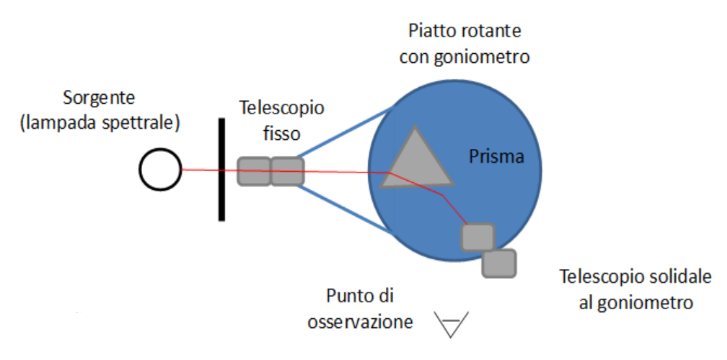
\includegraphics[scale = 0.5]{spettroscopio_prisma.png}
        \caption{Illustrazione dell'apparato spermentale utilizzato nella prima parte dell'esperienza.}
        \label{fig:prisma}
    \end{figure}
    \begin{table}[]
        \centering
        \begin{tabular}{cccc}
        colore&$ \lambda $[nm]&$\beta_i$&$\sigma_i $\\\hline\hline
        blu&467.8&$\ang{253.13\pm0.02}$&$\ang{-49.74\pm0.03}$\\
        azzurro&480.0&$\ang{253.37\pm0.02}$&$\ang{-49.5\pm0.03}$\\
        verde&508.6&$\ang{253.73\pm0.02}$&$\ang{-49.14\pm0.03}$\\
        rosso&643.8&$\ang{255.16\pm0.02}$&$\ang{-47.71\pm0.03}$\\\hline
        \end{tabular}
        \caption{Angoli di deflessione per le lunghezze d'onda osservate, misurati per la posizione di minima deflessione del prisma.}
        \label{tab:colori}
    \end{table}
    \newline
    In Fig.\ref{fig:lambda} riportiamo il grafico degli angoli di deflessione in funzione delle rispettive lunghezze d'onda.\newline
    Per procedere alla seconda fase si è quindi eseguito un fit lineare tramite la funzione:
    \begin{equation*}
    f(x) = ax+b
    \end{equation*}
    In tal modo abbiamo trovato i parametri che legano la lunghezza d'onda alla sua relativa deviazione, per il dato prisma.\newline
    Di seguito annotiamo i valori di best fit stimati:\newline\newline
    a = $(-600 \pm 11)$ nm$\cdot$rad\newline
    b = $(-0.740 \pm 0.002)$ rad\newline
    $\chi^2$ = 1.4\newline
    P-value = 0.51\newline
    
    \begin{figure}[h]
        \centering
        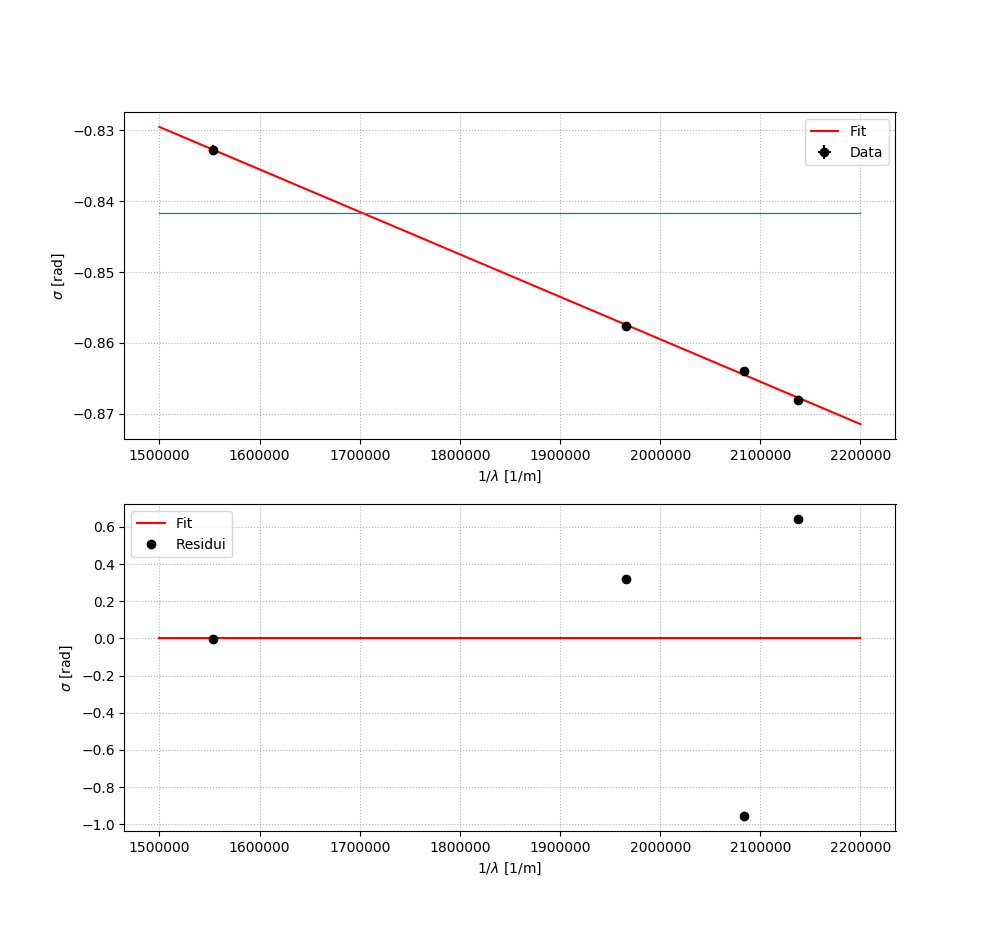
\includegraphics[scale = 0.5]{fit_prisma.png}
        \caption{\small Sopra: Grafico dell'angolo di deflessione in funzione della lunghezza d'onda, la linea blu indica l'angolo di deviazione della riga gialla del sodio.\newline Sotto: Grafico dei residui del fit.}
        \label{fig:lambda}
    \end{figure} 
    \newpage
\subsection*{Fase 2) Misura del doppietto del Sodio}
    In questa fase dell'esperimento abbiamo sostituito la lampada al cadmio con quella al sodio e dopo aver aspettato che si scaldasse, abbiamo misurato la posizione angolare della riga gialla:
    \begin{equation*}
    \delta_{Na}=\beta_{Na}-\beta_0=\ang{-48.22\pm0.03}
    \end{equation*}
    \noindent Quindi, utilizzando i valori stimati nella precedente fase, abbiamo stimato la lungheza d'onda di tale banda:
    
    \begin{equation*}
    \lambda_{Na} = 588 \pm 4 \, \mathrm{nm}\footnote{L'errore sulla lunghezza d'onda è stato stimato propagando l'errore della misura dell'angolo di deviazione, quelli dei due parametri di fit e tenendo conto della covarianza tra quest'ultimi.}
    \end{equation*}

\subsection*{Conclusioni}
La risoluzione dello spettroscopio a prisma, utilizzato in questa parte dell'esperienza, non ha reso possibile l'osservazione del doppietto giallo del sodio, tuttavia si è riusciti a misurare la lunghezza d'onda della riga visibile con un errore relativo dello $4/588\approx0.7\%$, i valori attesi sono: 589.592[nm] per una linea e 588.995[nm] per l'altra, entrambi entro una barra di errore dalla nostra misura. 

\section*{Misura della costante di Rydberg}

\subsection*{Fase 1) Misura del passo reticolare}
In questa parte dell'esperienza abbiamo utilizzato una lampada al mercurio. Inizialmente abbiamo preparato l'apparato sperimentale, regolando la posizione della lampada in modo tale da ottenere la massima intensità luminosa entrante nel primo telescopio e allineando quest'ultimo con il secondo mobile, per misurare lo zero angolare  ottenendo $\beta_0 = \ang{168.565 \pm 0.008}$. Infine si è posizionata la torretta con il reticolo di diffrazione.\footnote{Come errore sullo zero angolare si è preso il massimo tra la risoluzione dello strumento pari ad 1/120 di grado e la differenza tra le misure effettuate dai membri del gruppo.}
\newline Lo scopo di questa fase dell'esperienza è la stima del passo reticolare del reticolo. A tal fine abbiamo misurato l'angolo di riflessione totale $\theta_0$ e l'angolo di deflessione della riga verde del prim'ordine di rifrazione $\theta_1$, di cui abbiamo assunto nota la lunghezza d'onda $\lambda = 546.074\, \mathrm{nm}$. Da tali misure abbiamo potuto stimare il passo tramite la seguente formula:

\begin{equation}
    \mathrm{d} = \frac{\lambda}{\sin(\pi-\theta_0)-\sin(\theta_0-\theta_1)}
\end{equation}

\noindent$\theta_0 = \ang{36.44 \pm 0.02}$\newline
$\theta_1 = \ang{91.07 \pm 0.02}$\newline

\noindent Il  valore ottenuto è d = 1199.7 $\pm$ 0.6 [righe/mm] in accordo entro l'incertezza con il valore nominale di 1200 [righe/mm].

\newpage
\subsection*{Fase 2) Misura della costante di Rydberg}
In questa fase dell'esperienza è stata sostituita la lampada al mercurio con una all'idrogeno e sono stati misurati gli angoli di deflessione relativi alle righe osservate, mostrati in Tab.\ref{tab:r}:\footnote{Come errore sullo zero angolare si è preso il massimo tra la risoluzione dello strumento pari ad 1/120 di grado e la differenza tra le misure effettuate dai membri del gruppo.}

\begin{table}[h]
        \centering
        \begin{tabular}{ccc}
        colore&$ \lambda $[nm]&$\sigma_i $\\\hline\hline
        viola&433.8 $\pm$ 0.7&$\ang{82.78\pm0.02}$\\
        viola&435.1 $\pm$ 0.7&$\ang{82.88\pm0.02}$\\
        azzurro&486.0 $\pm$ 0.8&$\ang{86.69\pm0.02}$\\
        verde&533.6 $\pm$ 0.8&$\ang{90.17\pm0.02}$\\
        verde&544.1 $\pm$ 0.8&$\ang{90.93\pm0.02}$\\
        rosso&616.1 $\pm$ 0.9&$\ang{96.05\pm0.02}$\\
        rosso&656.6 $\pm$ 0.9&$\ang{98.88\pm0.02}$\\
        viola&434.4 $\pm$ 0.6&$\ang{113.51\pm0.02}$\\
        viola&437.1 $\pm$ 0.6&$\ang{113.89\pm0.02}$\\
        azzurro&486.5 $\pm$ 0.6&$\ang{120.77\pm0.02}$\\\hline
        \end{tabular}
        \caption{Angoli di deflessione per le lunghezze d'onda osservate.}
        \label{tab:r}
    \end{table}
    
\noindent I valori delle lunghezze d'onda, sono stati stimati tramite l'inversa della formula (1), utilizzando il valore precedetemente ricavato per il passo reticolare. \newline
Assunto che la serie di Balmer fosse quella che meglio descrive il range di lunghezze d'onda osservate, abbiamo individuato, usando il valore nominale della costante di Rydberg, e l'equazione (2), gli indici $\mathrm{n_2}$ che meglio approssimano le lunghezze d'onda osservate.
\begin{equation}
    \frac{1}{\lambda}=\mathrm{R}\biggl(\frac{1}{\mathrm{n_1^2}} - \frac{1}{\mathrm{n_2^2}}\biggr)
\end{equation}
Usando gli indici e le lunghezze d'onda che meglio vengono descritte dalle transizioni 2-3, 2-4 e 2-5 tra i livelli energetici si è eseguito un fit sui parametri della funzione (2) al fine di stimare la costante di Rydberg.\footnote{La funzione di fit utilizzata assumeva il valore della variabile $\mathrm{n}_1 = 2$ come costante} Riportiamo i dati nel grafico in Fig.\ref{fig:rydberg}; mentre i valori dei parametri ricavati dal fit sono:\newline\newline
    R = $(1.0967 \pm 0.0004)\times{10^7} \, \mathrm{m^{-1}}$\newline
    $\chi^2$ = 1.66\newline
    P-value = 0.202\newline
\begin{figure}[h]
    \centering
    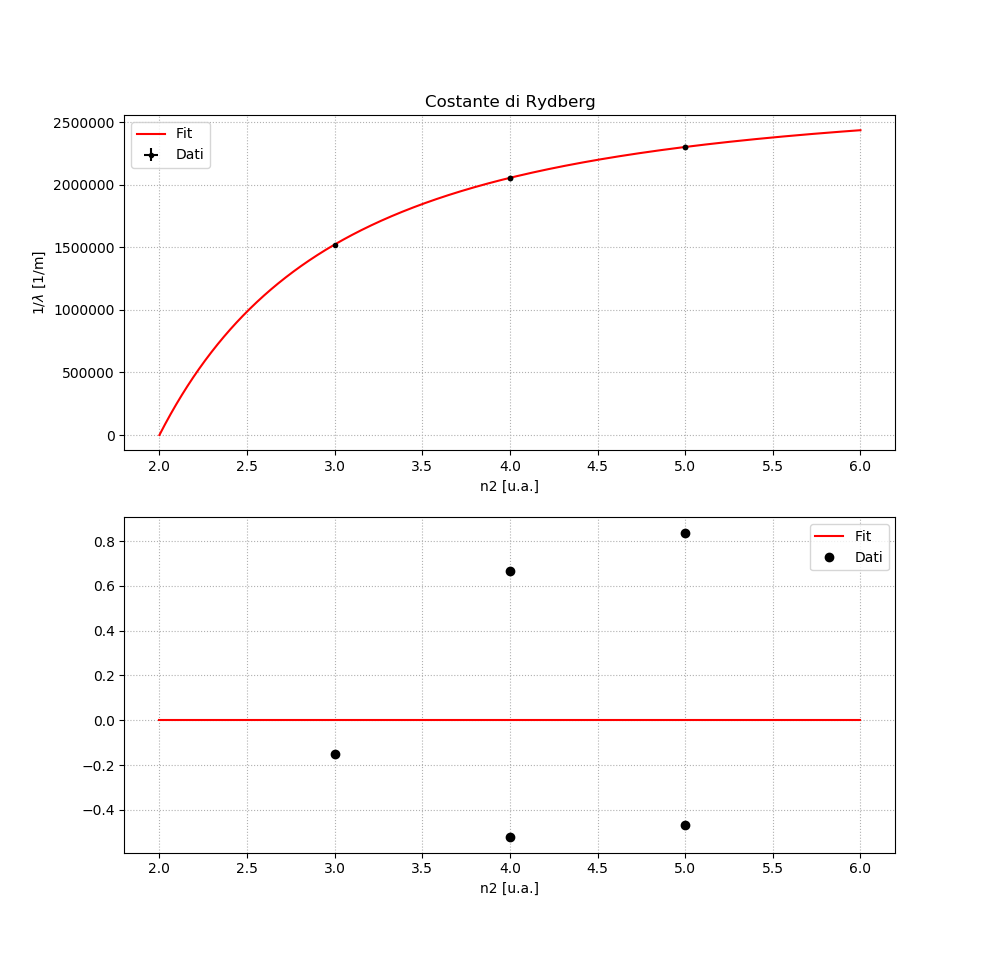
\includegraphics[scale = 0.35]{fig_rydberg.png}
    \caption{\small Sopra: Grafico dell'inverso della lunghezza d'onda in funzione di $\mathrm{n}_2$. Sotto: Grafico dei residui del fit.}
    \label{fig:rydberg}
\end{figure}

\subsection*{Fase 3) Misure del doppietto del Sodio}
Nella fase finale dell'esperienza si \`e sostituita la lampada ad idrogeno con quella a sodio,facendo sempre attenzione ad averla posizionata in modo da massimizzare l'intensità di luce entrante nell'apparato ottico. Abbiamo, quindi, osservato e misurato la deviazione angolare delle righe di emissione:\newline\newline
$\theta_1 =\ang{ 94.13 \pm 0.02}$\newline
$\theta_2 =\ang{ 94.16 \pm 0.02}$\newline\newline
Riportiamo le lunghezze d'onda stimate dalle misure:\newline\newline
$\lambda_1 = 588.9 \pm 0.3$ nm\newline 
$\lambda_2 = 589.4 \pm 0.3$ nm
\subsection*{Conclusioni}
La stima della costante di Rydberg per l'Idrogeno tramite fit dista una barra e mezzo d'errore dal valore atteso:\newline\newline
R$_{fit} = (1.0967 \pm 0.0004)\times{10^7}$\newline
R$_{att} = 1.0974 \times{10^7}$\newline\newline
Tale differenza potrebbe risultare dalla sottostima degli errori nella misura degli angoli. Per quantificare questa differenza assumiamo una distribuzione del parametro R$_{fit}$ gaussiana, con deviazione standard pari all'errore, si ha che la probabilità che R$_{fit}$ sia maggiore o uguale a R$_{att}$ risulta $\approx$ 5\% .\newline
Grazie al maggior potere risolutivo dello spettroscopio a reticolo, \`e possibile apprezzare la separazione angolare del doppietto del sodio e misurarne le rispettive lunghezze d'onda nel giallo. I valori stimati sono in accordo entro le incertezze con i valori attesi, in particolare:\newline
$\lambda_{prisma} = 588 \pm 4$ nm \newline
$\lambda_{1, reticolo} = 588.9 \pm 0.3$ nm\newline 
$\lambda_{2, reticolo} = 589.4 \pm 0.3$ nm\newline
$\lambda_{1, atteso} = 588.995$ nm\newline
$\lambda_{2, atteso} = 589.592$ nm

\noindent Da tali stime \`e possibile a posteriori definire un limite inferiore del potere risolutivo dello spettroscopio a prisma, che risulta essere maggiore a $\approx0.5$ nm.




















\section*{Dichiarazione}
I firmatari di questa relazione dichiarano che il contenuto della relazione \`e originale, con misure effettuate dai membri del gruppo, e che tutti i firmatari hanno contribuito alla elaborazione della relazione stessa.
\end{document}          